\documentclass[../ai_in_finance]{subfiles}
\usepackage[margin=1in]{geometry}
\usepackage{tikz}
\usetikzlibrary{positioning}
\usepackage{amsmath}
\usepackage{amssymb}
\usepackage{booktabs}
\usepackage{draftwatermark}

\SetWatermarkText{WSuo@Queensu.ca}
\SetWatermarkScale{1.4}
\SetWatermarkColor{gray!35}
\SetWatermarkAngle{45}

\usepackage{makeidx}
\makeindex

\begin{document}

\chapter{Introduction to Finance and AI}

\section{Why Finance Needs AI}\index{Why Finance Needs AI}

Finance is one of the most data-rich and decision-intensive domains in the modern economy. Financial institutions collect vast amounts of information every day, including prices, transactions, news, macroeconomic indicators, and firm-level reports. This information is often noisy, high-dimensional, and time-sensitive, which makes it difficult to analyze using simple rules or intuition alone.

At the same time, financial markets are highly competitive and dynamic. Firms, investors, and regulators all operate under pressure to make decisions quickly and accurately. As a result, methods from statistics, optimization, machine learning, and artificial intelligence have become increasingly important in tasks such as forecasting, risk management, trading, fraud detection, and customer service.

The central challenge in finance is not only to process data but also to make decisions under uncertainty. A portfolio manager must decide how much risk to take. A bank must estimate the probability of default. A regulator must detect suspicious behavior before losses become large. In each of these cases, the decision-maker needs a model, a framework for judgment, and an understanding of the incentives and constraints of the market.

A simple way to visualize this process is shown in Figure~\ref{fig:finance_ai_pipeline}: raw data feeds a model, the model's output is checked before being trusted, and only then does it inform an actual decision, a step this book returns to directly when discussing why models must be interpreted rather than worshipped.

\begin{figure}[htbp]
    \centering
    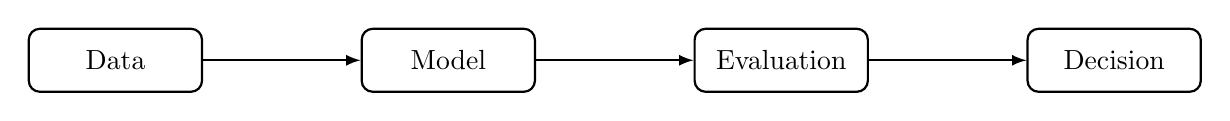
\begin{tikzpicture}[>=latex,thick,node distance=2.0cm]
        \node[draw,rounded corners,minimum width=2.2cm,minimum height=0.8cm] (data) {Data};
        \node[draw,rounded corners,minimum width=2.2cm,minimum height=0.8cm,right=of data] (model) {Model};
        \node[draw,rounded corners,minimum width=2.2cm,minimum height=0.8cm,right=of model] (eval) {Evaluation};
        \node[draw,rounded corners,minimum width=2.2cm,minimum height=0.8cm,right=of eval] (decision) {Decision};
        \draw[->] (data) -- (model);
        \draw[->] (model) -- (eval);
        \draw[->] (eval) -- (decision);
    \end{tikzpicture}
    \caption{A simple pipeline from financial data to modeling, evaluation, and finally decisions.}
    \label{fig:finance_ai_pipeline}
\end{figure}

There is also a strong economic reason for the growing role of AI in finance. Many financial decisions are made under limited information, time pressure, and changing conditions. Traditional rules may be too rigid to capture subtle patterns in the data. Machine learning methods can uncover nonlinear relationships and adapt to new information, provided they are used with appropriate domain knowledge and careful validation.

This book is about the intersection of finance and artificial intelligence. Its goal is to show how modern data-driven methods can be used to solve problems in finance while also explaining the logic behind those problems.

In practice, finance is not simply about making predictions from historical data. It is also about understanding incentives, constraints, and the consequences of decisions. A model that predicts a price movement may be useful, but it becomes much more valuable when it is linked to a trading rule, a risk limit, and an understanding of the costs of execution. Likewise, a credit model that predicts default must be interpreted in light of borrower behavior, contract terms, and broader macroeconomic conditions.

\section{A Short History of Quantitative Methods and AI in Finance}\index{Short History of Quantitative Methods and AI in Finance}

The idea of using mathematical models to make financial decisions is not new; what has changed over the past seventy years is the sophistication of the models and the scale of the data available to them. Tracing this history briefly helps explain why today's AI methods are best understood as the latest step in a long-running progression, not a sudden break from everything that came before.

The modern era of quantitative finance is often dated to 1952, when Harry Markowitz\index{Markowitz, Harry} formalized portfolio selection as an optimization problem over expected return and variance, work covered in depth in Chapter 10. This gave investors, for the first time, a rigorous mathematical language for the intuitive idea of diversification. The next major milestone came in 1973, when Fischer Black, Myron Scholes, and Robert Merton derived a closed-form formula for pricing options, the model introduced in Chapter 5, which turned derivatives trading from an informal, judgment-driven activity into something that could be systematically priced and hedged. Both developments shared a common feature: they used relatively simple, closed-form mathematics to capture an economically meaningful idea, and both remain in active use today despite decades of subsequent refinement.

The 1980s and 1990s saw the rise of algorithmic and electronic trading, as exchanges automated order matching and quantitative hedge funds began systematically exploiting statistical patterns in market data, foreshadowing the market microstructure and algorithmic trading material in Chapters 11 and 12. Around the same period, banks began applying statistical scoring models to credit decisions at scale, replacing purely judgment-based underwriting with models similar in spirit to the credit models in Chapter 9. Machine learning methods, decision trees, support vector machine\index{support vector machine (SVM)}s, and eventually gradient boosting\index{gradient boosting} and random forest\index{random forest}s, entered mainstream financial use in the 2000s and 2010s as computing power grew and larger datasets became available, expanding what had been simple statistical scoring into much richer pattern recognition, the subject of Chapter 6.

Since roughly 2015, two further developments have reshaped the field. Deep learning has made it practical to learn directly from large volumes of unstructured data, images, audio, and especially text, which is the foundation for the natural language processing methods in Chapter 14 and the alternative data methods in Chapter 15. And, more recently, large language model\index{large language model (LLM)}s have begun to be applied to tasks such as summarizing earnings calls, extracting structured information from filings, and supporting research workflows, an extension of the text-based methods in Chapter 14. Table~\ref{tab:history_timeline} summarizes this progression.

\begin{table}[htbp]
\centering
\caption{A brief timeline of quantitative methods in finance}
\label{tab:history_timeline}
\begin{tabular}{p{2.4cm}p{9.6cm}}
\toprule
Period & Development \\
\midrule
1950s & Markowitz mean-variance portfolio theory formalizes diversification mathematically \\
1970s & Black-Scholes-Merton\index{Black-Scholes-Merton Model} option pricing enables systematic derivatives pricing and hedging \\
1980s--1990s & Electronic exchanges and algorithmic trading; statistical credit scoring at scale \\
2000s--2010s & Machine learning (trees, ensembles, support vector machines) applied to prediction and classification tasks across finance \\
2015--present & Deep learning for unstructured data; large language models applied to financial text \\
\bottomrule
\end{tabular}
\end{table}

The throughline in this history is not that new methods replace old ones outright. Mean-variance optimization, Black-Scholes-Merton, and statistical scoring models are all still in daily use, often alongside the newer machine learning methods this book covers later. Each new wave of methods has instead expanded the range of problems that can be addressed and the amount of data that can be used, while the underlying economic questions, how to price risk, how to allocate capital, how to judge creditworthiness, have remained largely the same. This is a useful perspective to keep in mind throughout the book: a new AI technique is generally a new way of answering an old financial question, not a reason to discard the economic reasoning behind that question.

Table~\ref{tab:history_timeline}'s AI/ML rows compress six decades of a much older, independent field into two lines, ``machine learning applied to finance'' and ``deep learning and LLMs,'' which understates how much of that history had nothing to do with finance at all. AI and machine learning research has its own timeline, driven by its own breakthroughs and its own setbacks, long before most of it was ever pointed at a financial problem; Table~\ref{tab:ai_ml_timeline} traces that separate history on its own terms.

\begin{table}[htbp]
\centering
\caption{A timeline of key developments in AI and machine learning}
\label{tab:ai_ml_timeline}
\begin{tabular}{p{2.4cm}p{9.6cm}}
\toprule
Year & Development \\
\midrule
1956 & The Dartmouth Workshop\index{Dartmouth Workshop}, where John McCarthy and colleagues coin the term ``artificial intelligence,'' is widely regarded as the field's founding event \\
1958 & Frank Rosenblatt's Perceptron\index{Perceptron}, the first trainable artificial neural network, generates enormous early excitement \\
1969--1986 & Minsky and Papert's formal critique of the Perceptron's limitations helps trigger the first ``AI winter\index{AI Winter}'', a prolonged pullback in AI funding and research interest \\
1986 & Rumelhart, Hinton, and Williams popularize backpropagation\index{backpropagation}, an efficient algorithm for training multi-layer neural networks (Chapter 6) that ends the first AI winter \\
1997 & IBM's Deep Blue\index{Deep Blue} defeats reigning world chess champion Garry Kasparov, the first defeat of a sitting champion by a computer under tournament conditions \\
2012 & AlexNet\index{AlexNet}'s decisive win in the ImageNet\index{ImageNet} image-recognition competition demonstrates deep convolutional networks' advantage at scale, igniting the modern deep learning era (Chapter 15) \\
2016 & DeepMind's AlphaGo\index{AlphaGo} defeats Go champion Lee Sedol using deep reinforcement learning (Chapter 17), a game long assumed too complex for a computer to master \\
2017 & Vaswani et al.'s ``Attention Is All You Need'' introduces the transformer architecture\index{transformer architecture}, the foundation of every large language model that follows (Chapter 14) \\
2020 & OpenAI's GPT-3\index{GPT-3}, a 175-billion-parameter language model, demonstrates that scale alone unlocks broad, few-shot task performance \\
2022 & OpenAI's ChatGPT\index{ChatGPT} reaches mainstream adoption faster than any consumer software product before it, bringing generative AI into everyday use \\
\bottomrule
\end{tabular}
\end{table}

Two patterns stand out against Table~\ref{tab:history_timeline}. First, progress was not steady: the field's first AI winter shows that a technique's early promise (the Perceptron) can collapse under a well-founded technical critique and take over a decade to recover, a caution worth remembering whenever a new method arrives with confident claims attached. Second, essentially none of Table~\ref{tab:ai_ml_timeline}'s milestones were built for finance, Deep Blue plays chess, AlexNet classifies photographs, AlphaGo plays Go, yet each one supplied a general-purpose capability, pattern recognition at scale, sequential decision-making, language understanding, that finance adopted only after it had already been proven elsewhere. This is why Chapters 6, 14, 15, and 17 of this book introduce these same architectures and training algorithms largely as general-purpose machine learning, before turning to what makes each one specifically useful in a financial context.

\section{Who This Book Is For}\index{Who This Book Is For}

This book is written for readers who are quantitatively trained but may have little or no prior background in finance or economics. The intended audience includes students and practitioners with experience in mathematics, statistics, engineering, computer science, or data science who want to apply their skills in financial settings.

The book assumes familiarity with basic probability, statistics, calculus, and programming, especially Python. It does not assume prior knowledge of financial markets, accounting, or economic theory. Instead, each financial topic is introduced from the ground up and connected to the relevant mathematical and computational tools.

This approach is deliberate. Many quantitative readers are comfortable with optimization, regression, and probabilistic modeling, but they may not yet have developed the institutional intuition that is essential in finance. For example, a predictive model may be statistically impressive but still fail if it does not respect market frictions, incentives, and regulatory constraints. The book therefore emphasizes both mathematical methods and financial interpretation.

A useful way to think about this is that finance combines three layers of reasoning: economics, statistics, and implementation. Economics provides the structure of incentives and incentives-based behavior. Statistics provides tools for estimating uncertain relationships from data. Implementation addresses how a model behaves when it is embedded in a real system with costs, delays, and operational constraints. A strong finance practitioner must be fluent in all three.

\section{A Brief Introduction to Financial Markets}\index{Brief Introduction to Financial Markets}

A financial market is a place where financial assets are traded. These assets may include stocks, bonds, currencies, commodities, and derivatives. The purpose of these markets is to allow individuals, businesses, and governments to transfer capital, diversify risk, and price future uncertainty.

Financial markets do not exist only for speculation. They are a mechanism for allocating resources across time and across economic agents. A household may save for retirement. A firm may borrow to fund expansion. A government may issue debt to finance public spending. In each case, the market provides a way to connect those who have capital with those who need it.

The value of an asset is ultimately determined by the expectations of market participants about future cash flows, risk, and liquidity. For example, the price of a stock reflects the market's assessment of a firm's future profitability, while the price of a bond reflects expectations about default risk and interest rates. This makes finance a discipline that is both empirical and forward-looking.

Some of the most important financial institutions include banks, which intermediate between savers and borrowers; asset managers, which invest funds on behalf of clients; insurance companies, which protect against specific risks; exchanges, which provide platforms for trading; and regulators, which oversee market integrity and stability. Each of these institutions plays a distinct role in the functioning of the financial system, and their incentives shape the behavior of markets in subtle but important ways. Table~\ref{tab:market_institutions} summarizes these roles.

\begin{table}[htbp]
\centering
\caption{Major financial institutions and their roles}
\label{tab:market_institutions}
\begin{tabular}{p{4.0cm}p{8.0cm}}
\toprule
Institution & Role \\
\midrule
Banks & Intermediate between savers and borrowers \\
Asset managers & Invest funds on behalf of clients \\
Insurance companies & Protect against specific risks \\
Exchanges & Provide platforms for trading \\
Regulators & Oversee market integrity and stability \\
\bottomrule
\end{tabular}
\end{table}

Financial markets can be classified in several ways. Equity markets trade ownership claims in firms. Bond markets trade debt securities. Money markets trade short-term borrowing and lending instruments, typically with maturities under one year, and are covered in depth in Chapter 3. Derivatives markets trade contracts whose value depends on other assets. Foreign exchange markets trade currencies. Each market has its own structure, participants, and incentives. Table~\ref{tab:market_types} summarizes these market types.

\begin{table}[htbp]
\centering
\caption{Major types of financial markets}
\label{tab:market_types}
\begin{tabular}{p{4.0cm}p{8.0cm}}
\toprule
Market & What is traded \\
\midrule
Equity markets & Ownership claims in firms \\
Bond markets & Debt securities \\
Money markets & Short-term borrowing and lending instruments, such as Treasury bills, commercial paper, and repurchase agreements (Chapter 3) \\
Derivatives markets & Contracts whose value depends on other assets \\
Foreign exchange markets & Currencies \\
\bottomrule
\end{tabular}
\end{table}

A useful way to think about markets is through the roles of participants. Investors seek returns. Borrowers seek financing. Market makers provide liquidity by standing ready to buy and sell. Arbitrageurs exploit small pricing discrepancies. Regulators enforce rules and preserve confidence. These roles interact to create the price discovery process that makes markets informative. Table~\ref{tab:market_participant_roles} summarizes these participant roles.

\begin{table}[htbp]
\centering
\caption{Financial market participant roles}
\label{tab:market_participant_roles}
\begin{tabular}{p{4.0cm}p{8.0cm}}
\toprule
Participant & Objective or function \\
\midrule
Investors & Seek returns \\
Borrowers & Seek financing \\
Market makers & Provide liquidity by standing ready to buy and sell \\
Arbitrageurs & Exploit small pricing discrepancies \\
Regulators & Enforce rules and preserve confidence \\
\bottomrule
\end{tabular}
\end{table}

This perspective also helps explain why prices can move sharply even when the underlying news is limited. A market is not a single decision-maker but a collection of heterogeneous participants with different objectives, information sets, and time horizons. As a result, prices often reflect a balance of competing forces rather than a simple average of known facts.

\section{The Financial Data Ecosystem}\index{Financial Data Ecosystem}

Before turning to financial concepts, it is worth surveying the kinds of data that feed AI applications in finance, since different data types require different tools and different handling, and the rest of this book is organized in large part around them. Table~\ref{tab:data_types} summarizes the main categories.

\begin{table}[htbp]
\centering
\caption{Major categories of financial data}
\label{tab:data_types}
\begin{tabular}{p{2.6cm}p{9.4cm}}
\toprule
Data type & Description and examples \\
\midrule
Market data & Prices, quotes, trading volume, and order-book data, ranging from daily closing prices to microsecond-level tick data (Chapters 3, 11, 12) \\
Fundamental data & Accounting and financial statement data reported by firms, such as revenue, earnings, and balance sheet items (Chapter 4) \\
Macroeconomic data & Interest rates, inflation, unemployment, and other economy-wide indicators that affect asset prices broadly (Chapter 7) \\
Credit and transaction data & Loan repayment history, credit bureau data, and payment transaction records used in credit and fraud models (Chapters 9, 13) \\
Text and news data & Earnings call transcripts, news articles, analyst reports, and social media, used for sentiment and information extraction (Chapter 14) \\
Alternative data & Non-traditional sources such as satellite imagery, web traffic, or shipping data that proxy for economic activity (Chapter 15) \\
\bottomrule
\end{tabular}
\end{table}

Each data type has its own quality issues and its own conventions, and a recurring theme of this book is that using a data type well requires understanding where it comes from, not just how to load it into a model. Market data is timestamped and voluminous but expensive at high frequency and subject to microstructure noise (Chapter 2 introduces the basic handling of price and return data; Chapters 11 and 12 return to its highest-frequency form). Fundamental data is comparatively low-frequency and subject to reporting lag and accounting discretion, as Chapter 4 discusses in detail. Macroeconomic data is often revised after initial release, so a historical dataset built from final revised figures can overstate what was actually knowable in real time, a subtle look-ahead bias. Text and alternative data are the newest additions to the financial data ecosystem and, as Chapters 14 and 15 discuss, often require substantially more preprocessing before they are usable than the structured, tabular data that dominates the earlier chapters of this book.

A practical consequence of this variety is that a single financial AI system frequently combines several of these data types at once. A credit model might combine fundamental data about a small business with transaction data from its bank accounts and even satellite imagery of its physical location; a trading strategy might combine market data with sentiment extracted from news text. Building such combined systems is usually harder than building a single-data-type model, both because the data must be aligned in time and identity (the same firm, the same reporting period) and because each data source can fail or degrade independently.

\section{Core Financial Concepts}\index{Core Financial Concepts}

Before discussing AI applications, it is useful to understand a few central ideas in finance. These concepts provide the vocabulary and intuition needed to analyze financial problems, whether they are addressed with classical models or with modern machine learning techniques.

\subsection{Risk and Return}\index{Risk and Return}

A fundamental principle in finance is that higher expected return usually comes with higher risk. Investors must decide how much uncertainty they are willing to bear in exchange for potential reward. This tradeoff is central to portfolio choice, asset pricing, and corporate finance.

A simple illustration is shown in Figure~\ref{fig:risk_return_tradeoff}. Higher expected returns are typically obtained only by accepting greater variability in outcomes.

This tradeoff is one of the most important ideas in finance because it explains why investors do not simply choose the asset with the highest expected return. They must also consider whether the additional risk is acceptable given their objectives, constraints, and time horizon. The same logic appears in corporate finance, where firms must decide how much debt to use and how much uncertainty they can tolerate in their operations.

\begin{figure}[htbp]
    \centering
    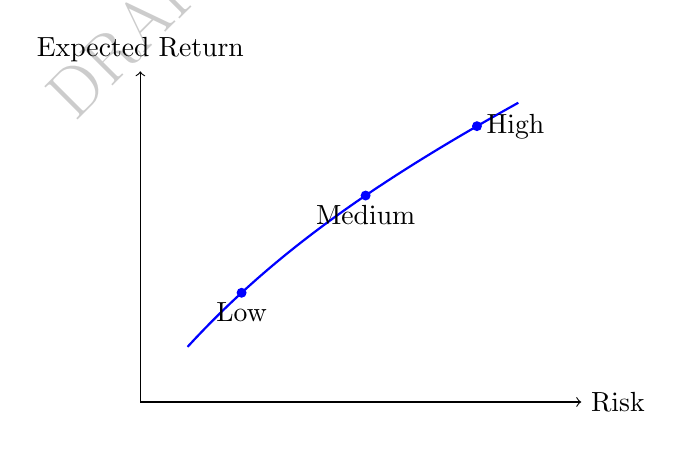
\begin{tikzpicture}[scale=1.0]
        \draw[->] (0,0) -- (5.6,0) node[right] {Risk};
        \draw[->] (0,0) -- (0,4.2) node[above] {Expected Return};
        \draw[blue,thick] (0.6,0.7) .. controls (1.7,1.9) and (3.0,2.8) .. (4.8,3.8);
        \fill[blue] (1.286,1.387) circle (1.8pt);
        \fill[blue] (2.861,2.622) circle (1.8pt);
        \fill[blue] (4.275,3.503) circle (1.8pt);
        \node[below] at (1.286,1.387) {Low};
        \node[below] at (2.861,2.622) {Medium};
        \node[right] at (4.275,3.503) {High};
    \end{tikzpicture}
    \caption{The risk-return tradeoff: higher expected returns generally require accepting greater risk.}
    \label{fig:risk_return_tradeoff}
\end{figure}

\subsection{Time Value of Money}\index{Time Value of Money}

Money available today is worth more than the same amount in the future because it can be invested and earn returns. This principle underlies discounting, present value, interest rates, and valuation. In practice, this means that future cash flows must be converted into present value terms before they can be compared fairly. This process is central to bond pricing, project valuation, and investment analysis.

The future value of an amount $PV$ invested today at rate $r$ for $n$ years is 
$$FV = PV(1+r)^n,$$
 and Table~\ref{tab:tvm_table} applies this formula to \$1,000 invested at three different rates over three different horizons.

\begin{table}[htbp]
\centering
\caption{Future value of \$1,000 invested at different rates and horizons}
\label{tab:tvm_table}
\begin{tabular}{lrrr}
\toprule
Annual rate & 10 years & 20 years & 30 years \\
\midrule
3\% & \$1,343.92 & \$1,806.11 & \$2,427.26 \\
6\% & \$1,790.85 & \$3,207.14 & \$5,743.49 \\
9\% & \$2,367.36 & \$5,604.41 & \$13,267.68 \\
\bottomrule
\end{tabular}
\end{table}

Two patterns in Table~\ref{tab:tvm_table} are worth internalizing because they recur throughout the book. First, compounding is highly nonlinear in the rate: doubling the rate from 3\% to 6\% more than doubles the 30-year future value, and tripling it to 9\% multiplies the 30-year value by more than five. Second, the horizon matters enormously: at 9\%, the difference between a 10-year and a 30-year horizon is a factor of roughly 5.6, even though the annual rate never changed. Present value, used constantly from Chapter 5 onward, is simply this same relationship read in reverse: 
$$PV = \frac{FV}{(1+r)^n},$$
discounting a future amount back to today.

\subsection{Diversification}\index{Diversification}

Diversification refers to spreading investments across different assets or risks to reduce the effect of any single loss. The intuition is simple: not all investments move in the same way at the same time. In portfolio construction, diversification is a way to reduce idiosyncratic risk while retaining exposure to broad economic factors.

\subsection{Market Efficiency}\index{Market Efficiency}

The efficient market hypothesis\index{Efficient Market Hypothesis (EMH)} suggests that asset prices reflect available information to a large extent. This idea has important consequences for forecasting, trading, and the interpretation of abnormal returns. Although markets are not perfectly efficient at all times, this framework remains a core reference point in finance.

For quantitative readers, this idea is particularly important because it motivates the distinction between signal extraction and noise. If prices already incorporate most information quickly, then generating simple excess returns may be difficult. This does not mean that all opportunities disappear, but it does mean that the relevant question is often not whether a signal exists, but whether it survives transaction costs, model risk, and market frictions.

In this sense, market efficiency is not a statement that no one can ever beat the market. Rather, it is a reminder that profitable strategies must overcome several obstacles, including competition from other informed participants, delays in data availability, and the costs of trading.

\section{Financial Problems That AI Can Help Solve}\index{Financial Problems That AI Can Help Solve}

AI is useful in finance because many important problems involve prediction, classification, optimization, and decision-making under uncertainty. In practice, these problems appear in forecasting asset prices or returns, predicting credit default or bankruptcy, detecting fraudulent transactions, optimizing portfolios, identifying trading opportunities, and extracting information from financial text and news. In each case, the financial problem is not merely a generic data problem. The underlying financial model, market structure, and regulatory context matter. For example, a credit model must reflect the economics of default, while a trading strategy must account for transaction costs, market liquidity, and execution risk.

This is a key point for readers with a machine learning background. A model that performs well in a generic prediction task may fail in finance if it ignores institutional details. A fraud detector may need to understand customer behavior and regulatory requirements. A pricing model may need to respect no-arbitrage conditions. In other words, finance is not just a collection of datasets; it is a structured domain with economic logic and constraints.

As a simple illustration, suppose a bank wants to predict whether a borrower will default on a loan. A purely statistical model may use historical repayment behavior and demographic variables, but a useful financial model must also consider the borrower’s debt burden, income stability, collateral, and macroeconomic conditions. The best solution is often a combination of economic reasoning, statistical estimation, and machine learning.

The same principle applies to asset pricing, portfolio optimization, and trading. A forecasting model may perform well in sample but still fail in practice if it ignores transaction costs, liquidity constraints, or changes in market regimes. This is why finance requires both predictive accuracy and economic plausibility.

It is also important to recognize that financial data are often generated by strategic behavior. When a firm announces earnings, when a central bank changes interest rates, or when a large investor enters the market, the data reflect not only economic fundamentals but also the reactions of many agents. This makes financial modeling both statistical and behavioral in nature.

Table~\ref{tab:problem_taxonomy} organizes the main problem types this book addresses by the kind of machine learning task involved and points to where each is covered in depth, giving a preview of the book's structure from a problem-first, rather than chapter-first, perspective.

\begin{table}[htbp]
\centering
\caption{A taxonomy of AI problem types in finance}
\label{tab:problem_taxonomy}
\begin{tabular}{p{2.6cm}p{6.0cm}p{2.4cm}}
\toprule
Task type & Example financial problem & Covered in \\
\midrule
Regression & Forecasting returns, volatility, or a credit spread & Ch.~6, 7 \\
Classification & Predicting default, fraud, or a trading signal's direction & Ch.~6, 9, 13 \\
Time series forecasting & Forecasting interest rates, volatility, or macro indicators & Ch.~7 \\
Optimization & Constructing a portfolio subject to risk and constraint limits & Ch.~10 \\
Clustering / dimensionality reduction & Grouping similar firms or compressing a large factor set & Ch.~6, 10 \\
Sequential decision-making & Executing a trade over time to minimize impact & Ch.~11, 12 \\
Natural language processing & Extracting sentiment or information from text & Ch.~14 \\
Anomaly detection & Flagging unusual transactions or account behavior & Ch.~13 \\
\bottomrule
\end{tabular}
\end{table}

Two things stand out from this taxonomy. First, several finance problems map onto more than one machine learning task type, portfolio construction, for example, is fundamentally an optimization problem but often uses regression or dimensionality reduction as an input, which is why later chapters frequently combine methods from Chapter 6 with domain-specific structure. Second, some columns of Table~\ref{tab:problem_taxonomy} recur across many chapters (classification appears in credit, trading, and fraud contexts) precisely because the underlying statistical machinery, introduced once in Chapter 6, is reused throughout the rest of the book rather than re-derived for each application.

\section{How This Book Is Organized}\index{How This Book Is Organized}

This book is designed to introduce finance and AI in a layered way. The early chapters focus on financial foundations so that readers without a background in the subject can build intuition. Later chapters introduce machine learning and statistical methods, followed by applications in areas such as risk management, portfolio management, trading, and compliance.

The progression is deliberate. The book begins with the basic language of finance, then moves to the mathematical tools used to analyze financial data. After that, it introduces classical financial models, such as portfolio theory and credit risk models, before extending them with modern AI techniques. This structure is intended to help readers build intuition first and then connect that intuition to more advanced methods.

The structure of the book is intentionally progressive. It begins by introducing financial concepts in plain language, then develops the mathematical and statistical tools needed to analyze them, before turning to classical financial models and finally to AI-based extensions. This sequence allows readers to understand the economic logic of a problem before applying more advanced methods to it. Practical case studies and exercises are woven throughout so that the reader can connect theory with application and see how these ideas behave in realistic settings.

By the end of this chapter, the reader should have a broad understanding of what finance is, why it is data-rich, how markets function, and why AI methods must be interpreted in light of financial theory and institutional structure. These ideas provide the foundation for the more technical chapters that follow.

A compact summary of the book's conceptual flow is shown in Figure~\ref{fig:book_flow}.

\section{Notation and Conventions Used in This Book}

A few notational conventions are used consistently across chapters, and stating them once here avoids repetition later. Random variables and their realizations are both written in italics (for example, $X$ or $x$), with the distinction clear from context. A hat denotes an estimate, so $\hat\beta$ is an estimated coefficient and $\hat y$ is a predicted value, as opposed to $\beta$ and $y$, which denote the true, generally unobserved, parameter and outcome. Vectors and matrices are written in bold only where the distinction from scalars is not otherwise clear from context, and $\|\cdot\|$ denotes the Euclidean norm. Time subscripts are written as $X_t$, with $t-1$ denoting the immediately preceding period, and 
$$\Delta X_t = X_t - X_{t-1}$$
denoting a first difference.

Monetary amounts are given in US dollars unless stated otherwise, and percentages are used interchangeably with decimals (5\% and 0.05 mean the same thing) depending on which is clearer in context. Interest rates, returns, and growth rates are annualized unless a different frequency (monthly, daily) is explicitly stated. Every chapter's worked numerical examples are also reproduced, and were originally verified, in that chapter's companion Jupyter notebook, so that a reader can check any computation in the text by running the corresponding notebook cell rather than only reading the printed result.

Each chapter follows the same template: an opening motivation, several sections of theory interleaved with at least one fully worked numerical example, a section on the practical challenges of the chapter's topic, a short list of key takeaways, a set of suggested exercises, and a further reading list of standard textbooks for readers who want to go deeper than a single chapter allows. Figures are simple schematic diagrams rather than photographs or screenshots, and are meant to organize ideas rather than to substitute for the surrounding prose.

\section{Financial Statements, Cash Flows, and Valuation}\index{Financial Statements, Cash Flows, and Valuation}

Although much of modern finance is expressed through prices, rates, and stochastic models, the underlying economic reality is often much simpler: firms create value by generating cash flows over time. A company can be profitable on paper and still face financial distress if it does not generate enough cash to meet obligations. For this reason, financial analysis begins with a careful reading of financial statements, especially the balance sheet, the income statement, and the cash flow statement.

The balance sheet summarizes what a firm owns and what it owes at a point in time. Assets include cash, inventories, property, and intellectual property. Liabilities include debt, payables, and other obligations. Equity represents the residual claim of owners after liabilities are accounted for. The income statement shows revenues, expenses, and profit over a period of time. The cash flow statement, by contrast, explains how cash moved through the business and is often more informative than accounting earnings when one is trying to understand solvency and future financing needs.

This distinction is important because accounting profits and economic value are not identical. A firm may report large earnings while consuming cash through inventory accumulation, capital expenditure, or working capital needs. For investors and lenders, the question is not only whether the firm appears profitable, but whether it can sustain operations and meet future obligations. Data-driven methods in finance are often built around exactly this type of economic interpretation. A predictive model may forecast earnings, but a financial analyst must also ask whether those earnings are backed by cash generation and durable competitive advantages.

The concept of valuation rests directly on this logic. The value of an asset is the present value of the expected future cash flows that it will generate, discounted at an appropriate rate. In symbols, a simple present value relation is

\begin{equation*}
V = \sum_{t=1}^{T} \frac{CF_t}{(1+r)^t},
\end{equation*}
where $CF_t$ denotes the cash flow in period $t$ and $r$ is the discount rate. This expression is one of the most important ideas in finance because it unifies bond pricing, stock valuation, project appraisal, and many forms of corporate analysis. The challenge is that future cash flows are uncertain and the discount rate must reflect both time and risk. This is where statistics and econometrics become essential.

In practice, valuation is rarely a purely mechanical exercise. Firms face changing competitive conditions, regulatory pressure, and shifts in investor sentiment. A company with strong historical performance may still lose value if its market position erodes or if interest rates rise sharply. This is why financial models are most useful when combined with qualitative judgment. A model can estimate probabilities or forecast trends, but it cannot replace the need to understand the business model, the industry structure, and the incentives of management.

This point is especially relevant for AI applications in finance. A machine learning model may forecast revenues or defaults with impressive accuracy, but it should not be deployed blindly. The output should be checked against the firm's accounting structure, its debt obligations, and the economic context in which it operates. The best systems therefore combine statistical learning with financial reasoning and careful validation.

\section{Why Finance Is Not Just a Collection of Numbers}\index{Why Finance Is Not Just a Collection of Numbers}

A common misconception is that finance is simply the manipulation of numerical data. In reality, finance is about incentives, contracts, and the allocation of resources under uncertainty. The numbers that appear in financial statements or market data are the outcomes of institutional processes. They emerge from decisions about borrowing, investing, pricing, regulation, and risk management.

For this reason, a quantitative analyst should not be satisfied with a high-performing prediction model unless there is also a clear economic explanation for why the model works. If a model identifies a pattern in stock returns, that pattern may reflect risk exposure, information diffusion, transaction costs, or temporary market inefficiency. If a model predicts default, it may be capturing leverage, deteriorating cash flow, or sector-level stress. In each case, the signal is meaningful only when interpreted through the lens of finance.

This is also why financial modeling must be careful about causality. Correlation is not enough. A variable may be associated with future returns or defaults for reasons that do not persist once market conditions change. A sensible finance practitioner therefore tests assumptions, monitors model stability, and remains aware of regime shifts. AI can help discover patterns, but good financial judgment is needed to decide whether those patterns are economically plausible and practically useful.

\section{A Practical Perspective on the Role of AI in Finance}\index{Practical Perspective on the Role of AI in Finance}

The purpose of AI in finance is not to replace financial expertise. It is to augment it. AI methods can process large and complex data sources, detect nonlinear patterns, and automate tasks that would be too time-consuming for humans. However, the usefulness of these methods depends on the quality of the problem formulation. A poorly defined objective can lead to a model that looks sophisticated but produces poor decisions.

Consider the example of credit scoring. A bank may want to estimate the probability that a borrower will default over the next year. A machine learning model can use many variables, including repayment history, income, occupation, and account activity. Yet the model will be most useful when it is tied to domain knowledge about loan structure, collateral, legal obligations, and the macroeconomic environment. Otherwise, it may learn patterns that reflect temporary conditions rather than durable credit risk.

The same principle applies to portfolio construction, fraud detection, and market forecasting. The rational use of AI in finance requires an appreciation of uncertainty, costs, and incentives. It also requires humility. Even sophisticated models can fail when the environment changes, when data quality is poor, or when market participants adapt to the model itself.

This augmentation-not-replacement view also has organizational consequences that are easy to overlook in a purely technical treatment. Deploying an AI system in a financial institution typically requires sign-off from risk management, compliance, and sometimes a model validation team whose job is specifically to challenge the model before it is used with real capital or real customers, a process often called model risk management\index{model risk management}. A model that cannot be explained to these stakeholders, regardless of its statistical performance, is often not deployable at all, which is part of why Chapter 16 treats explainability as a first-class technical requirement rather than an afterthought. Readers coming from a pure machine learning background sometimes find this institutional layer frustrating, since it can slow down the deployment of a model that performs well in backtesting. It is best understood, however, as a reflection of the fact that a financial model's errors are rarely private: a mispriced loan, a bad trade, or a missed fraud case can affect customers, counterparties, and, in aggregate, the stability of the financial system as a whole, which is precisely why financial AI is regulated more heavily than AI applied to, say, recommending movies.

\section{Connecting the Foundations to Later Chapters}\index{Connecting the Foundations to Later Chapters}

The ideas introduced in this chapter provide the conceptual foundation for the more technical material that follows. Once the reader understands why markets exist, how assets are valued, and what kinds of institutions shape financial decisions, the later chapters on statistics, risk, trading, and machine learning will be easier to appreciate. The central theme is that financial problems are not just mathematical problems. They are problems of economic reasoning under conditions of uncertainty, constraints, and strategic behavior.

This perspective is essential for anyone who wants to work at the intersection of finance and AI. A successful practitioner must be able to translate a financial question into a statistical problem, then translate the output of a model back into a financial decision. That translation requires both technical skill and financial intuition.

\begin{figure}[htbp]
    \centering
    
\begin{tikzpicture}[>=latex,thick,node distance=2.2cm]
        \node[draw,rounded corners,minimum width=3.0cm,minimum height=0.9cm,align=center] (finance) {Financial\ Foundations};
        \node[draw,rounded corners,minimum width=3.0cm,minimum height=0.9cm,right=of finance,align=center] (stats) {Statistical\ Methods};
        \node[draw,rounded corners,minimum width=3.0cm,minimum height=0.9cm,right=of stats,align=center] (ai) {AI and\ Applications};
        \draw[->] (finance) -- (stats);
        \draw[->] (stats) -- (ai);
    \end{tikzpicture}
    \caption{The book progresses from finance fundamentals to statistical tools and then to AI-driven applications.}
    \label{fig:book_flow}
\end{figure}

\section{Finance as a System of Incentives and Information}\index{Finance as a System of Incentives and Information}

A striking feature of finance is that the objects being analyzed are not merely numbers but the outcomes of incentives. A manager may be rewarded for short-term earnings growth even when that growth is not sustainable. A lender may extend credit to a borrower who appears safe in normal conditions but becomes fragile when conditions deteriorate. A regulator may face pressure to support market confidence even when this increases moral hazard. These examples show that finance is deeply intertwined with human behavior and institutional design.

The consequence is that even the best statistical model must be interpreted in context. A pattern in the data may reflect genuine economic structure, but it may also reflect the incentives of agents who produced the data. Financial data are therefore not passive observations. They are records of strategic interaction. This is a major reason why quantitative work in finance is never purely mechanical.

In many settings, information is dispersed across many participants. A single investor may know a small piece of the truth; markets aggregate these pieces through prices. This is one reason why price data are so valuable. They encode information about expectations, beliefs, and constraints. Yet they also encode noise, strategic behavior, and market frictions. The task of the analyst is therefore to separate signal from noise while remembering that the data themselves are generated by participants with incentives.

Two well-documented historical episodes illustrate how badly things can go wrong when a model is deployed without enough attention to the incentives shaping the underlying data. In the years leading up to the 2008 financial crisis, statistical models of mortgage default risk were built on historical data from a period of rising home prices and relatively loose underwriting standards. Those models implicitly assumed that the incentives generating the historical data, in particular, that mortgage originators bore meaningful consequences for making bad loans, would continue to hold. In practice, the rise of mortgage securitization changed those incentives: many originators sold loans onward quickly enough that they bore little of the eventual default risk themselves, so underwriting quality quietly deteriorated in ways the historical default models never observed. The models were not statistically wrong in a narrow sense; they were estimated correctly on the data available. They were wrong because the economic process generating the data had shifted underneath them, exactly the non-stationarity concern flagged elsewhere in this chapter and developed further in Chapter 9.

A second, smaller-scale illustration is the phenomenon of Goodhart's Law\index{Goodhart's Law}, often summarized as ``when a measure becomes a target, it ceases to be a good measure.'' A credit score, for example, is originally a statistical summary that correlates with creditworthiness. But once borrowers and lenders both know that a specific numerical threshold controls loan approval or pricing, some participants will alter their behavior specifically to cross that threshold, for reasons that may or may not reflect a genuine change in creditworthiness. This is a direct example of the reflexivity theme introduced in Chapter 6: unlike a model of a physical system, a financial model's targets can adapt to the existence of the model itself, which is one more reason financial AI systems require ongoing monitoring rather than a one-time validation.

\section{Uncertainty, Probability, and Decision-Making}\index{Uncertainty, Probability, and Decision-Making}

Finance is fundamentally about decisions under uncertainty. A lender does not know with certainty whether a borrower will repay. An investor does not know whether an asset price will rise or fall. A firm does not know whether a new project will be profitable. The relevant question is not whether uncertainty can be eliminated, because it usually cannot. The relevant question is how decision-makers should act when outcomes are uncertain and when the costs of being wrong are not symmetric.

It is worth being precise about what kind of not-knowing this actually is, since finance regularly runs into two quite different flavors. The economist Frank Knight\index{Knight, Frank} drew this distinction sharply in 1921: \emph{risk} describes a situation where the possible outcomes are known and their probabilities can be estimated, whether from a well-understood physical process (a fair coin) or from a long, stable history of similar past events, while \emph{uncertainty} (sometimes called Knightian uncertainty\index{Knightian uncertainty}) describes a situation where even the set of possible outcomes, let alone their probabilities, cannot be fully specified in advance. A casino game is risk in this precise sense; a genuinely novel financial crisis, a first-of-its-kind fraud scheme, or a new technology's effect on an entire industry is uncertainty. This distinction matters well beyond a single introductory paragraph: nearly every probabilistic model in this book, the Value at Risk models of Chapter 8, the credit-scoring models of Chapter 9, the volatility forecasts of Chapter 7, implicitly treats its subject as risk, assuming that a historical sample is enough to pin down the relevant probabilities, when the actual situation may still contain a meaningful component of genuine Knightian uncertainty that no amount of historical data can fully resolve. Keeping this distinction in mind is a useful, low-cost habit throughout the rest of this book: before trusting a model's probability estimate, it is worth asking whether the situation is closer to a repeatable game with a stable, estimable distribution, or closer to a genuinely novel situation where the model's confidence may be misplaced.

This is where probability and expected value become central. If an investor faces two possible outcomes, a gain and a loss, the expected value of the gamble may be positive even if the investor would prefer not to take the risk. This distinction motivates the idea of risk aversion. A risk-averse decision-maker usually requires a larger expected payoff to accept a gamble with greater uncertainty. This logic underlies portfolio choice, corporate financing, and insurance.

A simple expression for expected value is

\begin{equation*}
\mathbb{E}[X] = \sum_i p_i x_i,
\end{equation*}
where $p_i$ is the probability of state $i$ and $x_i$ is the associated payoff. This equation is simple, but it captures a profound idea: decision-making in finance requires combining possible outcomes with their probabilities. The challenge is that probabilities are rarely known with perfect precision, and the environment can change. For this reason, financial models must be updated as new information arrives and assessed against outcomes that are not fully predictable.

A small numerical example makes the idea of risk aversion concrete. Suppose an investor is offered a gamble with a 50\% chance of gaining \$20,000 and a 50\% chance of losing \$10,000. The expected value of the gamble is
\begin{equation*}
\mathbb{E}[X] = 0.5(20{,}000) + 0.5(-10{,}000) = \$5{,}000,
\end{equation*}
which is positive, so a risk-neutral decision-maker, one who cares only about expected value, should accept it. Yet many investors would decline this gamble, because the possibility of losing \$10,000 matters more to them than the expected value calculation alone suggests. Economists capture this with a concave utility function $u(\cdot)$, so that the investor evaluates the gamble using expected utility, $\mathbb{E}[u(X)]$, rather than expected value directly. The certainty equivalent\index{Certainty Equivalent} is the guaranteed amount that gives the same expected utility as the gamble; for a risk-averse investor, the certainty equivalent is always less than the \$5,000 expected value, and the gap between the two, sometimes called the risk premium, is a direct measure of how much the investor is willing to pay to avoid uncertainty.

Making this concrete requires choosing a specific utility function and applying it to the investor's total wealth, not just the gamble's payoff in isolation, since a concave function is only meaningful evaluated at actual wealth levels. Suppose the investor's wealth today is $W_0 = \$50{,}000$, and, following the square-root utility function $u(W) = \sqrt{W}$, a standard textbook example of a risk-averse (concave) utility function. The gamble leaves the investor with wealth $W_0 + 20{,}000 = \$70{,}000$ or $W_0 - 10{,}000 = \$40{,}000$, so
\begin{equation*}
\mathbb{E}[u(W)] = 0.5\sqrt{70{,}000} + 0.5\sqrt{40{,}000} \approx 0.5(264.575) + 0.5(200.000) = 232.288.
\end{equation*}
The certainty equivalent wealth $CE$ solves $u(CE) = \mathbb{E}[u(W)]$, that is, $\sqrt{CE} = 232.288$, giving $CE \approx \$53{,}957.51$, noticeably less than the expected wealth of $0.5(70{,}000) + 0.5(40{,}000) = \$55{,}000$. The risk premium is the difference,
\begin{equation*}
\text{Risk premium} = \$55{,}000 - \$53{,}957.51 \approx \$1{,}042.49,
\end{equation*}
which has a direct interpretation: this investor would accept a guaranteed $\$53{,}957.51$ in place of the gamble, meaning they would pay up to $\$1{,}042.49$ to avoid the gamble's uncertainty entirely, even though the gamble's expected wealth is higher. This same logic, comparing an uncertain payoff to its certainty equivalent, underlies the pricing of insurance, the equity risk premium, and the risk-return tradeoff introduced earlier in this chapter, and it reappears in a more technical form as the reason a risk-averse portfolio manager accepts a lower expected return in exchange for lower volatility in the mean-variance framework of Chapter 10.

\subsection*{The Kelly Criterion: How Much to Bet, Not Just Whether}\index{Kelly criterion}

A positive expected value answers whether a favorable gamble is worth taking at all, but a repeatable opportunity, place the same favorable bet over and over, raises a second, sharper question a single certainty-equivalent calculation does not: what \emph{fraction} of current wealth should be wagered each time? Betting too little leaves genuine edge on the table; betting too much, this section's next result shows, can make an investor with a real, positive edge poorer with certainty over time.

The reason this question is nontrivial, rather than simply ``bet as much as a positive edge allows,'' is that wealth wagered repeatedly compounds rather than accumulates. A single bet's expected value is an arithmetic average across outcomes, and it is exactly the right tool for deciding whether to take that bet once. But wealth carried across many repetitions is a product of per-round multipliers, $(1+f)$ after a win and $(1-f)$ after a loss, not a sum of per-round gains, and a quantity built from repeated multiplication is governed by its \emph{geometric} mean, not its arithmetic one. The two can disagree sharply: a single large enough loss multiplies surviving wealth by a factor close to zero, and no number of favorable multiplications afterward fully reverses that, so a bet size can raise the arithmetic average of outcomes while simultaneously driving the geometric average, and with it long-run wealth, toward zero. This asymmetry, not risk aversion in the subjective sense discussed above, is what makes betting too large a fraction ruinous even when every individual bet retains positive expected value, and it is exactly what the growth-rate result below makes precise.

The Kelly criterion answers this precisely for a repeatable bet with probability $p$ of winning (paying $b$ dollars per dollar wagered) and probability $q=1-p$ of losing the full amount wagered: the fraction of wealth that maximizes the long-run \emph{geometric} growth rate of wealth is
\begin{equation*}
f^* = p - \frac{q}{b}.
\end{equation*}
For an even-money bet ($b=1$) with a $60\%$ win probability, $f^* = 0.6 - 0.4 = 0.2$: wager exactly $20\%$ of current wealth on each repetition, no more and no less.

The reason ``no more'' matters as much as ``no less'' is the genuinely surprising part. The long-run growth rate of wealth from repeatedly wagering a fraction $f$ is $g(f) = p\ln(1+f) + q\ln(1-f)$; evaluating it at three candidate fractions for this same $60\%$-favorable bet,
\begin{equation*}
g(0.2) \approx 0.0201, \qquad g(0.5) \approx -0.0340, \qquad g(1.0) = -\infty,
\end{equation*}
shows that wagering half of wealth on every repetition, despite each individual bet still having positive expected value, produces a \emph{negative} long-run growth rate: an investor following this rule is mathematically certain to see their wealth decay toward zero over enough repetitions, not merely experience higher volatility around a still-positive trend. Wagering everything each time ($f=1$) is worse still, guaranteed eventual ruin, since a single loss (probability $q=0.4$ on any given bet, and probability 1 eventually across enough repetitions) wipes out the entire stake with nothing left to bet with afterward. This is a sharper, more quantitative version of the risk-aversion lesson above: a decision-maker who evaluates only a single bet's expected value, without asking how large a fraction of wealth to commit to it when it repeats, can be led toward a sizing decision that is not just uncomfortable but ruinous, exactly the kind of position-sizing discipline that resurfaces, in a portfolio context rather than a single repeated bet, in Chapter 10's discussion of leverage and Chapter 11's execution-sizing decisions.

\subsection*{The Value of Information: What Is a Perfect Signal Worth?}\index{Value of information}

A closely related question asks not how much to bet, but how much a decision-maker should be willing to pay for information that resolves uncertainty \emph{before} a decision is made. Suppose a firm is deciding whether to fund a \$2 million project, an idealized version of the kind of capital-budgeting decision Chapter 4 develops in far more detail. The project succeeds with probability $0.4$, returning a net gain of \$5 million, or fails with probability $0.6$, losing the full \$2 million invested. Without any additional information, the expected value of proceeding is
\begin{equation*}
E[\text{Proceed}] = 0.4(5) + 0.6(-2) = \$0.8 \text{ million},
\end{equation*}
positive, and better than the \$0 from not proceeding at all, so a rational, risk-neutral firm proceeds, accepting the $60\%$ chance of a \$2 million loss along with the $40\%$ chance of a \$5 million gain.

Now suppose the firm could instead consult a perfectly accurate forecaster, at some price, who reveals with certainty which state (success or failure) will occur before the firm must commit. Knowing this, the firm would proceed only in the success state and decline in the failure state, earning
\begin{equation*}
E[\text{Proceed} \mid \text{perfect information}] = 0.4(5) + 0.6(0) = \$2.0 \text{ million},
\end{equation*}
since the \$2 million loss is avoided entirely in the $60\%$ of cases where failure would otherwise have occurred. The expected value of perfect information (EVPI)\index{Expected Value of Perfect Information (EVPI)} is the difference between these two figures,
\begin{equation*}
\text{EVPI} = 2.0 - 0.8 = \$1.2 \text{ million},
\end{equation*}
the absolute maximum a rational firm should be willing to pay for a perfectly accurate signal before deciding, since paying any more would make consulting the forecaster worse than simply proceeding blind. In practice, no real forecast, credit model, or market signal is perfectly accurate, so EVPI is best understood as an upper bound: it answers ``how much could better information possibly be worth here,'' a question worth asking explicitly before investing in additional data, a more sophisticated model, or a costly due-diligence process, exactly the kind of cost-benefit judgment call that recurs, applied to specific data vendors and model types, throughout this book's later chapters.

\section{Bayesian Updating: Learning from New Information}\index{Bayesian Updating: Learning from New Information}

A closely related idea, and one that underlies how many machine learning systems in this book are best interpreted, is that beliefs about an uncertain quantity should be updated, not replaced, as new evidence arrives. Bayes' theorem\index{Bayes' theorem} formalizes this:
\begin{equation*}
\Pr(A \mid B) = \frac{\Pr(B \mid A)\,\Pr(A)}{\Pr(B)},
\end{equation*}
where $\Pr(A)$ is the prior probability of some hypothesis $A$ before seeing evidence $B$, $\Pr(B\mid A)$ is the likelihood of observing that evidence if $A$ is true, and $\Pr(A\mid B)$ is the posterior probability of $A$ after accounting for the evidence.

A concrete example, directly relevant to the fraud detection material in Chapter 13, shows why this matters. Suppose 1\% of transactions at a bank are fraudulent, so $\Pr(\text{Fraud}) = 0.01$. A fraud detection model correctly flags 95\% of actual fraud, $\Pr(\text{Flag}\mid\text{Fraud}) = 0.95$, but also flags 3\% of legitimate transactions, $\Pr(\text{Flag}\mid\text{Not Fraud}) = 0.03$. Given that a transaction has been flagged, what is the probability it is actually fraudulent? Applying Bayes' theorem,
\begin{eqnarray*}
\Pr(\text{Flag}) &=& \Pr(\text{Flag}\mid\text{Fraud})\Pr(\text{Fraud}) + \Pr(\text{Flag}\mid\text{Not Fraud})\Pr(\text{Not Fraud})\\
& =& 0.95(0.01) + 0.03(0.99) \\
&=& 0.0392, \\
\Pr(\text{Fraud}\mid\text{Flag}) &=& \frac{0.95(0.01)}{0.0392} \approx 0.242.
\end{eqnarray*}
Despite a model that sounds highly accurate (95\% detection, only 3\% false alarms), a flagged transaction is fraudulent only about 24\% of the time, because genuine fraud is so rare that even a small false-positive rate produces many more false alarms than true detections in absolute terms. This is the same base-rate intuition behind the discussion of imbalanced classification in Chapter 6, and it is a direct, quantitative illustration of why accuracy alone, discussed qualitatively earlier in this chapter, is a poor way to evaluate a model applied to a rare event.

Bayesian updating also describes, at a conceptual level, how a well-run financial model should be maintained over time. Rather than treating a model's parameters as fixed forever, or discarding a model entirely the first time it makes a mistake, a Bayesian perspective treats each new batch of data as an opportunity to revise a belief incrementally: the posterior from today becomes the prior for tomorrow's update. This is the same spirit behind the model-monitoring loop discussed later in this chapter, and behind the state-space and Kalman-filtering methods introduced formally in Chapter 7, which are, in effect, Bayesian updating carried out recursively over time.

The ``posterior becomes the next prior'' idea is easiest to see by continuing the fraud example one step further. Suppose the flagged transaction above is now compared against the customer's typical spending location, and this second, independent signal shows the transaction occurred somewhere the customer has never transacted before, a pattern that occurs in 60\% of genuine fraud cases but only 10\% of legitimate ones: $\Pr(\text{Unusual Location}\mid\text{Fraud}) = 0.6$ and $\Pr(\text{Unusual Location}\mid\text{Not Fraud}) = 0.1$. Rather than starting over, a Bayesian analysis treats the first posterior, $\Pr(\text{Fraud}\mid\text{Flag}) \approx 0.242$, as the prior for this second update:
\begin{eqnarray*}
\Pr(\text{Location}) &=& 0.6(0.242) + 0.1(1-0.242) = 0.221, \\
\Pr(\text{Fraud}\mid\text{Flag},\text{Location}) &=& \frac{0.6(0.242)}{0.221} \approx 0.657.
\end{eqnarray*}
Two independent pieces of weak-to-moderate evidence, an automated flag and an unusual location, combine to raise the probability of fraud from a 1\% base rate to roughly 66\%, each update using exactly the same formula with the previous posterior in place of the original prior. Figure~\ref{fig:bayesian_chain} lays out this chain of updates directly. This is precisely how a production fraud system in Chapter 13 accumulates evidence from several independent model outputs before deciding whether a transaction warrants manual review, and it is why an ensemble of several weak signals, evaluated one Bayesian update at a time, can be more reliable than any single signal considered alone.

\begin{figure}[htbp]
    \centering
    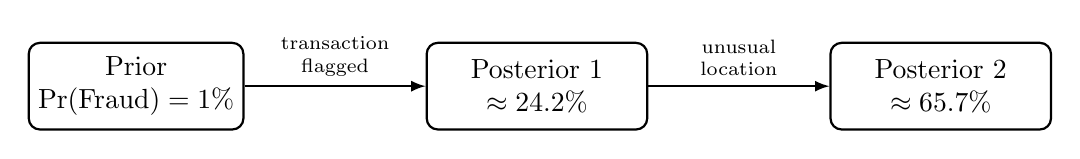
\begin{tikzpicture}[>=latex,thick,node distance=2.3cm]
        \node[draw,rounded corners,align=center,minimum width=2.6cm,minimum height=1.1cm] (prior) {Prior\\$\Pr(\text{Fraud})=1\%$};
        \node[draw,rounded corners,align=center,minimum width=2.8cm,minimum height=1.1cm,right=of prior] (post1) {Posterior 1\\$\approx24.2\%$};
        \node[draw,rounded corners,align=center,minimum width=2.8cm,minimum height=1.1cm,right=of post1] (post2) {Posterior 2\\$\approx65.7\%$};
        \draw[->] (prior) -- node[above,align=center,font=\scriptsize] {transaction\\flagged} (post1);
        \draw[->] (post1) -- node[above,align=center,font=\scriptsize] {unusual\\location} (post2);
    \end{tikzpicture}
    \caption{Sequential Bayesian updating on the fraud example: each new, independent piece of evidence turns the previous posterior into the next prior, using the identical Bayes'-theorem formula both times.}
    \label{fig:bayesian_chain}
\end{figure}

\section{Why Models Must Be Interpreted, Not Worshipped}\index{Why Models Must Be Interpreted, Not Worshipped}

A common temptation in finance is to trust a model too much simply because it is sophisticated or produces attractive historical results. Such overconfidence is dangerous. A model can be mathematically elegant and still be economically misleading. A stock prediction model may perform well for a while and then fail when market conditions change. A credit model may appear accurate in a stable period and become unstable during a recession. A fraud model may detect obvious anomalies but miss subtle forms of misconduct that change over time.

Figure~\ref{fig:finance_ai_pipeline}'s pipeline already named the reason this matters: the evaluation step between a model and the decision it informs is not a formality, it is where an overconfident model gets caught, or does not.

This is why model evaluation in finance is not just a statistical exercise. It is also an economic and operational exercise. The relevant questions are not only whether the model fits the data but whether its assumptions make sense, whether its outputs are usable, and whether the implementation is robust. Finance rewards humility. The best practitioners understand both the strengths and the limits of their methods.

The 1998 collapse of Long-Term Capital Management\index{Long-Term Capital Management (LTCM)} (LTCM), a hedge fund whose partners included two Nobel laureates in economics and whose models were, by the standards of the time, extremely sophisticated, is a case study in exactly this failure mode, examined in more detail in Chapter 3. The fund's models had correctly estimated how various fixed-income spreads behaved under historically normal conditions, but had no mechanism for anticipating a regime in which several previously uncorrelated markets, including Russian sovereign debt, moved together in a global flight to quality, at the same moment the fund's own highly leveraged positions made it a forced seller into a market with too few buyers. No later chapter's model, however statistically sophisticated, is exempt from this same risk: a model is only ever as good as the range of conditions it was built and tested to anticipate, which is precisely why the stress-testing and scenario-analysis techniques covered in Chapter 8 exist as a check on quantitative models generally, not a specialized technique reserved for portfolio risk alone.

\section{Challenges of Applying AI in Finance}

Before moving into the technical chapters, it is worth naming, at a high level, the recurring challenges that will resurface throughout this book whenever AI methods are applied to financial problems. Later chapters revisit each of these in much greater depth and with concrete techniques for addressing them.

\textbf{Data challenges.} Financial data are noisy, unevenly sampled, subject to reporting delays, and sometimes revised after the fact. Historical datasets can also suffer from survivorship bias, in which failed firms or discontinued strategies are quietly excluded, making the past look more favorable than it actually was.

\textbf{Non-stationarity.} Unlike many physical systems, financial markets change their own statistical behavior over time, in response to new regulation, new technology, changing investor composition, and the actions of other market participants, including the actions of other AI systems. A model calibrated\index{calibration} on one period can therefore fail in the next, even without any error in how it was built.

\textbf{Overfitting\index{overfitting} and backtest illusions.} Because financial data are limited relative to the number of strategies and features that can be tried, it is easy to find a pattern that worked well in history purely by chance. A strategy that looks excellent in a backtest can perform poorly, or lose money, once deployed with real capital.

\textbf{Interpretability and accountability.} Many financial decisions, particularly credit and insurance decisions, are subject to legal requirements that they be explainable and non-discriminatory. This constrains how opaque a model can be, regardless of its statistical performance, and is examined in depth in Chapter 16.

\textbf{Operational and execution frictions.} A model's statistical output is not the same as a financial outcome. Transaction costs, market impact\index{market impact}, latency, and operational failures can all erode or eliminate a theoretical edge, which is why economic evaluation, not just statistical evaluation, is emphasized throughout this book.

\textbf{Ethical and systemic considerations.} Widely adopted AI models can create correlated behavior across many market participants, potentially amplifying booms and busts. Models used in lending, insurance, or hiring can also encode or amplify existing biases in historical data if they are not carefully audited.

These are not reasons to avoid AI in finance. They are reasons to apply it carefully, with an understanding of financial institutions, incentives, and market structure alongside statistical skill, which is precisely the combination this book aims to build.

\section{Case Vignette: How Classical Finance and AI Combine in Practice}\index{How Classical Finance and AI Combine in Practice}

To make the abstract themes of this chapter concrete, consider a stylized (fictional) example that previews how the pieces of this book fit together. Suppose a mid-sized asset manager wants to build a systematic equity strategy that selects stocks likely to outperform over the coming quarter.

The manager does not start with machine learning. The process begins with the financial statement analysis of Chapter 4: screening a universe of firms on fundamentals such as profitability, leverage, and cash generation, discarding firms with clear signs of financial distress before any prediction model is involved. This step encodes economic reasoning, distress and financial weakness are meaningful even before considering whether a stock's price is likely to rise, that a purely data-driven model applied to raw price history would not automatically discover.

Next, the manager builds a predictive model, using the regression and classification tools of Chapter 6, to rank the remaining firms by expected relative performance. The model's features draw on several of the data types catalogued in Table~\ref{tab:data_types}: fundamental ratios from the statement-screening step, momentum and volatility measures computed from the time series methods of Chapter 7, and, increasingly, sentiment scores extracted from earnings-call transcripts using the natural language processing methods of Chapter 14. Critically, the model is evaluated with the walk-forward methodology described later in this book, not a random train-test split, since a random split would let the model see information from the future relative to some of its training data.

The ranked predictions then become an input to portfolio construction, not the final answer. Chapter 10's mean-variance and factor-based methods convert a raw ranking into a set of position sizes that respect diversification, risk limits, and transaction cost constraints, since the highest-ranked stock in isolation might be too risky, too illiquid, or too correlated with the rest of the portfolio to hold at a large weight. Finally, before any trade is placed, the execution considerations of Chapter 11 determine how to actually buy and sell the resulting positions without moving prices adversely, and the risk models of Chapter 8 continuously monitor whether the realized portfolio is behaving as expected.

At every step in this vignette, a classical financial concept, distress screening, portfolio diversification, transaction costs, sits alongside a modern statistical or machine learning method, and neither one is sufficient on its own: the machine learning ranking without financial screening risks recommending distressed firms with temporarily attractive statistical patterns, while financial screening without machine learning would leave the manager unable to process the scale of fundamental, price, and text data available. This interleaving of classical and modern methods, not the replacement of one by the other, is the organizing principle of every applied chapter that follows.

\section{Key Takeaways}

The key lesson of this chapter is that finance is a domain in which data, uncertainty, and decision-making interact closely. Quantitative readers can make rapid progress in the subject by connecting mathematical tools with financial intuition, but they must also learn to interpret models in light of market structure, incentives, and institutional constraints. AI methods are most useful in finance when they are guided by sound financial reasoning rather than used as black-box tools. In short, the most effective applications of AI in finance combine statistical skill, economic understanding, and practical judgment.

Several more specific points from this chapter are worth carrying forward explicitly. The history in Section 1.2 showed that today's machine learning methods extend, rather than replace, decades of classical quantitative finance, which is why nearly every applied chapter in this book pairs a classical model with a modern one instead of presenting the modern method alone. The data ecosystem in Section 1.5 previewed the range of data types, market, fundamental, macroeconomic, credit, text, and alternative, that later chapters draw on, each with its own quality issues. The numerical examples in this chapter, compounding in Table~\ref{tab:tvm_table}, the gamble and certainty equivalent, and the fraud-detection application of Bayes' theorem, were chosen because each illustrates a principle (nonlinearity of compounding, risk aversion, and the danger of ignoring base rates) that reappears in a more technical form in a later chapter. Finally, the case vignette in Section 1.19 is worth revisiting after finishing the book: a reader who initially finds the asset-management example abstract should be able to return to it once Chapters 4, 6, 7, 10, 11, and 14 have been covered and see exactly how each step would be implemented in practice.

\section{Suggested Exercises}

\begin{enumerate}
    \item Define the difference between risk and uncertainty in the context of financial decision-making.
    \item Explain why the time value of money matters for investment decisions.
    \item List three types of financial markets and describe the assets traded in each.
    \item Give one example of a financial problem where AI could be useful and one where classical statistical methods might be sufficient.
    \item Write a short paragraph explaining why financial models should still be considered when using machine learning in finance.
    \item Describe one financial institution and explain how it connects savers, borrowers, or investors.
    \item Discuss why a model that performs well in a generic prediction task may still fail in a financial setting.
    \item A gamble offers a 60\% chance of gaining \$8,000 and a 40\% chance of losing \$5,000. Compute the expected value, and explain, using the concept of a certainty equivalent, why a risk-averse investor might still reject it even though the expected value is positive.
    \item Pick two of the challenges listed in Section 1.18 (``Challenges of Applying AI in Finance'') and describe a concrete financial scenario, not already used in the chapter, in which that challenge could cause an AI-based system to fail.
    \item Using Table~\ref{tab:tvm_table}, compute the future value of \$5,000 invested for 20 years at 6\%, and verify your answer is consistent with scaling the \$1,000 figure in the table.
    \item A disease-screening test correctly identifies 90\% of people who have a rare disease affecting 0.5\% of the population, and has a 5\% false-positive rate. Using Bayes' theorem as in Section 1.16, compute the probability that a person who tests positive actually has the disease, and explain why the result is counterintuitive.
    \item Choose one entry from Table~\ref{tab:problem_taxonomy} and explain, in a short paragraph, why the financial problem you chose could plausibly be framed as more than one of the task types listed in the table (regression, classification, optimization, and so on).
    \item Pick one milestone from Table~\ref{tab:history_timeline} and explain, using material from later in this chapter, why the newer methods that followed it did not make it obsolete.
    \item Continuing the sequential Bayesian updating example in Section 1.16, suppose a third, independent signal arrives: the transaction amount is a round number (e.g., exactly \$500), a pattern present in 40\% of fraud cases but only 15\% of legitimate ones. Using $\Pr(\text{Fraud}\mid\text{Flag},\text{Location}) \approx 0.657$ as the new prior, compute the updated posterior probability of fraud after all three signals, and comment on how quickly the probability approaches certainty as independent evidence accumulates.
    \item Using the Kelly criterion, compute the optimal betting fraction $f^*$ for an even-money bet with a $70\%$ win probability, and compute the long-run growth rate $g(f)$ at $f^*$ and at $f=0.9$, commenting on whether betting nearly everything is ever justified even when the win probability is this favorable.
    \item A firm is deciding whether to enter a new market at a cost of \$3 million. Entry succeeds with probability $0.3$, returning a net gain of \$12 million, or fails with probability $0.7$, losing the full \$3 million. Compute the expected value of entering, the expected value under perfect information, and the resulting EVPI, and explain what the firm should conclude if a market-research report claiming near-perfect accuracy costs \$4 million.
\end{enumerate}

\section{Further Reading}

For readers who want to deepen their understanding of the financial ideas introduced in this chapter, the following texts are useful starting points:

\begin{itemize}
    \item Brealey, Myers, and Allen, \emph{Principles of Corporate Finance}. A comprehensive introduction to corporate financial decision-making, including the time-value-of-money and valuation ideas this chapter introduces at a conceptual level and Chapter 5 develops formally.
    \item Hull, \emph{Options, Futures, and Other Derivatives}. The standard reference for derivatives pricing; useful background for the brief history of Black-Scholes-Merton option pricing sketched in this chapter's timeline and covered in full in Chapter 5.
    \item Bodie, Kane, and Marcus, \emph{Investments}. Covers portfolio theory, market efficiency, and the risk-return tradeoff introduced qualitatively in this chapter, previewing the quantitative treatment in Chapter 10.
    \item Campbell, Lo, and MacKinlay, \emph{The Econometrics of Financial Markets}. A rigorous treatment of the statistical methods used to test market efficiency and analyze financial time series, going well beyond this chapter's introductory discussion.
    \item Goodfellow, Bengio, and Courville, \emph{Deep Learning}. The standard reference for the deep learning methods behind the large language model and unstructured-data applications previewed in this chapter's history section and covered in Chapters 14 and 15.
    \item Chan, \emph{Machine Trading}. A practitioner-oriented introduction to building and testing systematic trading strategies, extending the case vignette in this chapter into the algorithmic trading material of Chapters 11 and 12.
\end{itemize}

These references cover foundational finance, asset pricing, and the use of quantitative methods in financial applications.

\end{document}
